\subsection{Les interfaces}
\label{subsec:interfaces}
Une interface est un ensemble de méthodes et de propriétés qui définissent un contrat. Une classe qui implémente une interface doit alors implémenter toutes les méthodes et propriétés de cette interface. Cela permet de définir une structure très générique qui sera utilisée, ensuite, par les classes que nous définirons. 

\UPSTIaRetenir{Les interfaces permettent de définir un contrat que les classes qui les implémentent doivent respecter. La déclaration d'une interface se fait de manière similaire à la déclaration d'une classe, mais aucune méthode n'est implémentée.}
\lstDeleteShortInline~
\begin{UPSTIactivite}[][Exemple d'interface]
    \UPSTIquestion{Donner un exemple dans lequel l'utilisation d'une interface est pertinente, par exemple dans le monde du jeu vidéo. Expliquer}
    \vspace{5cm}
\end{UPSTIactivite}

\begin{UPSTIinfor}{Les interfaces sous CodeSys}
    \begin{minipage}{.7\linewidth}
        Sous CodeSys, une interface s'ajoute dans l'arborescence du projet en utilisant l'outil \emph{Add Object}. Il suffit alors de sélectionner le type de l'objet à ajouter (interface) et de le nommer. Elle apparaît alors ainsi que les méthodes et propriétés qui lui sont associées. 
        
        Le mot clef utilisé sous CodeSys est \lstinline{INTERFACE}.


        Le mot clef \lstinline{IMPLEMENT} est utilisé lors de la déclaration d'une classe pour indiquer que cette classe implémente une interface.


        
    \end{minipage}
    \hfill
    \begin{minipage}{.25\linewidth}
        \centering
        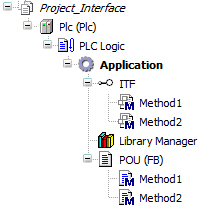
\includegraphics[width=\linewidth]{_cds_img_itf_method.png}
    \end{minipage}

\end{UPSTIinfor}

\paragraph{Dans notre contexte} les interfaces pourront définir, pour un ensemble de blocs fonctionnels : 
\begin{itemize}
    \item Des propriétés (\lstinline{PROPERTY})
    \begin{itemize}
        \item Nom
        \item Type
        \item Accesseurs
    \end{itemize}
    \item Des méthodes (\lstinline{METHOD})
    \begin{itemize}
        \item Nom
        \item Paramètres d'entrées et de sorties (\lstinline{VAR_INPUT}, \lstinline{VAR_OUTPUT}, \lstinline{VAR_IN_OUT})
    \end{itemize}
\end{itemize}

\begin{UPSTIinfor}{Plusieurs interfaces}
    Une classe peut implémenter plusieurs interfaces. Elle devra alors implémenter toutes les méthodes et propriétés de ces interfaces.

    \begin{lstlisting}
FUNCTION_BLOCK <fb_name> IMPLEMENTS <ITF_name_0> |, <ITF_name_1> |, <ITF_name_n>
    \end{lstlisting}
\end{UPSTIinfor}

%%% TODO : Ajouter les interfaces comme groupe homogène (slides 13-14) %%%